\documentclass[twoside, 12pt]{article}

%----------All packages loaded-----------
\usepackage[utf8]{inputenc}
\usepackage{geometry}
\usepackage{hyperref}
\usepackage{fancyhdr}
\usepackage{enumitem}
\usepackage[english]{babel}
\usepackage{csquotes}
\usepackage{graphicx}
\usepackage{listings}
\usepackage{amsmath}
\usepackage{amssymb}
\usepackage{mathtools}
\usepackage[bibnewpage]{apacite}
\usepackage{accents}


%--------------------------------------------------------------

%----------------A couple of setups------------
\hypersetup{colorlinks=true, linkcolor=blue, filecolor=black, urlcolor=black, citecolor=blue}
\urlstyle{same}
\geometry{a4paper,total={170mm,246.2mm},left=20mm,top=25.4mm}
\linespread{1.25}
\numberwithin{equation}{section}
\newcommand{\ubar}[1]{\underaccent{\bar}{#1}}
%--------------------------------------------------------------

%-------Headers and footers---
\pagestyle{fancy}

\fancyhead{}

\fancyhead[LO]{\scriptsize KOEN VERBRUGGEN 2016}
\fancyhead[RO]{\footnotesize \thepage}
\fancyhead[LE]{\footnotesize \thepage}
\fancyhead[RE]{\scriptsize THE DESIGN OF THE LENDER OF LAST RESORT}

\fancyfoot{}

\renewcommand{\footnoterule}{%
  \kern -3pt
  \hrule width 20mm height 0.5pt
  \kern 2pt
}
%\renewcommand*\footnoterule{}
\renewcommand{\headrulewidth}{0pt}
%-------------------------------------------------------------

%--------------Titel en auteurs-------------------------------
\title{\vspace{-15mm} The Design of the Lender of Last Resort: A theoretical approach}
\author{Koen Verbruggen\footnote{MSc Economics student at Tilburg University. ANR: 459785, E-mail: \href{mailto:k.l.p.verbruggen@tilburguniversity.edu}{k.l.p.verbruggen@uvt.nl}.} }

\begin{document}

%----------Begin van het document met titel etc.---------------
\date{February 29, 2016}
\maketitle

\fancypagestyle{firststyle}{\fancyhf{}\fancyfoot{}\fancyhead{}\renewcommand{\headrulewidth}{0pt}}
\thispagestyle{firststyle}

\section{Repullo's optimal allocation of LLR responsibilities}\label{sec:modelrepullo}
In this section we are going to use the model of \cite{repullo2000} to address the optimal allocation of LLR responsibilities between a central bank and the DI. Besides this it is also discussed who should be in charge of bank supervision.

The model consists of three periods. In period 1 a bank raises an amount of deposits normalized to 1. All these deposits are invested in an illiquid asset that yields a random return $\widetilde{R}$ at $t=2$. Asymmetric information hinders that the assets can be sold at $t=1$, although it is possible to liquidate the bank at $t=1$\footnote{Other banks do not know the quality of the assets invested in, causing difficulties to sell them at their actual worth.}. Deposits are fully insured by a DI and can be withdrawn at $t=1$ or $t=2$.

At $t=1$ a fraction of the deposits $v \in (0,1)$ are withdrawn. Since there is no market for the illiquid assets the bank is holding, it cannot sell these to pay out the withdrawals. Therefore it will be forced into liquidation unless it can borrow from the LLR. Two government agencies can fulfill the role of LLR. The central bank and the DI. To act as LLR the chosen agency is given supervision power to gather information about the assets of the bank. This leads to a signal $u \in (0,1)$ at $t=1$ that contains information about the expected return of the illiquid asset in period $t=2$. This can be described as follows:
\begin{equation}\label{eq:repulloreturn}
  \widetilde{R}=\begin{cases}
    0, & \text{with probability 1-u}.\\
    R, & \text{with probability u}.
  \end{cases}
\end{equation}
where $R>1$.

It is important to mention that $u$ is not publicly observed and therefore non-verifiable. It is only known to the supervisor who evaluates the bank. The two agencies both maximize their objective functions in which they care about their own expected final wealth net of bankruptcy costs in the event of a bank failure. The bankruptcy costs are denoted by $c$ and reflect administrative costs of closing the bank and negative externalities associated with a bank failure. The two agencies might have different views on supporting a bank or not. Two reasons exist for this difference: (1) the DI needs to compensate depositors if the bank fails, while the central bank does not have this liability and (2) the central bank and the DI have different fractions of the bankruptcy costs that they incur.

\subsection{Optimal LLR policy}
Starting with the benchmark case where $u$ is verifiable for everyone and no agency is therefore involved in doing research to find out what this value is. The expected return of the illiquid asset net of expected bankruptcy costs are compared with the liquidation value $L$ net of bankruptcy costs $c$:
\begin{equation}\label{eq:a}
uR-(1-u)c \geq L-c
\end{equation}

If the expected return to the bank's assets net of expected bankruptcy costs are bigger than the liquidation value net of optimal bankruptcy costs, it is optimal to provide liquidity. That is, if:
\begin{equation}\label{optimalrepullo}
u\geq u^*= L/(R+C)
\end{equation}
If observed $u$ is equal to $u^*$, both sides are equal and society is indifferent between saving the bank or letting it fail.

\subsection{Central bank as LLR}
Suppose the central bank is the LLR and after observing $u$ it has to decide to support the bank by lending funds equal to the amount of withdrawals or let it fail. In $t=2$ two situations can occur, one is that the realized return is $R$ and the central bank receives back the loan outstanding or $R=0$ and the central bank loses the amount $v$ and there is a bankruptcy cost. The central bank has the following cost function if it supports the bank:
\begin{equation}
(1-u)v+(1-u)\beta c
\end{equation}
The cost if the central bank does not support the bank is simply $\beta c$.

The central bank will compare the two cost functions and the central bank will support the bank if:
\begin{equation}\label{eq6}
u\geq \hat{u}(v)=\frac{v}{v+\beta c}
\end{equation}
The minimum $u$ for which the bank is granted loans depends on $v$. $\hat{u}$ is increasing in the amount of withdrawals. In \autoref{fig:RepCB} the optimal $u^*$ is compared to $\hat{u}$.

\begin{figure}[htbp]
\begin{centering}
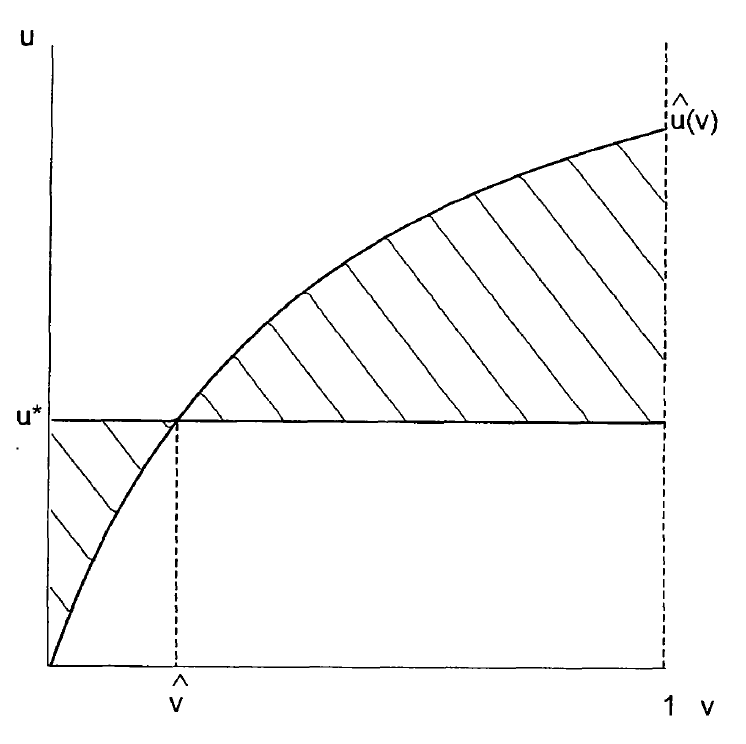
\includegraphics[width=8cm]{RepulloCB2000.png}
\caption{The central bank as LLR. Source: \protect\cite{repullo2000}.}
\label{fig:RepCB}
\end{centering}
\end{figure}

This graph shows that to the left of $\hat{v}$ the central bank is too soft. It also supports banks for which a lower $u$ is observed than $u^*$, to the right of $\hat{v}$ the central bank is too tough. the intuition behind this graph is quite straightforward. When the amount of withdrawals is very small the central bank has an incentive to support the bank, because if it does not the bank fails with probability 1 and the central bank incurs the bankruptcy cost $\beta c$. If it supports the bank the expected costs if $v$ is very small are equal to $(1-u)\beta c$, obviously if $v$ is large the central bank takes on more risk and demands a higher $u$.

\subsection{Deposit insurance corporation as LLR}
Next we turn to the case where the DI acts as LLR. Again after observing the signal $u$ it has to decide whether to lend the bank the amount of withdrawals or let it fail. The biggest change is that the DI also takes into account the fact that in case of liquidation it has to pay $1-v$ to the remaining depositors and incurs a share $\gamma$ of the bankruptcy costs. This gives the following cost function when the DI supports the bank:
\begin{equation}
(1-u)(v+(1-v)+(1-u)\gamma c
\end{equation}
On the other hand if the DI lets the bank go into bankruptcy, it also has to pay the deposits minus the liquidation value of the bank $1-L$. So not supporting the bank gives the following cost function:
\begin{equation}
(1-L)+\gamma C
\end{equation}
Again the LLR will support the bank if the cost of supporting are lower than letting it fail. That is, if: 
\begin{equation} \label{eq8}
u\geq \bar{u}= \frac{L}{1+\gamma c}
\end{equation}
$\bar{u}$ is the $u$ that makes the cost of both decisions equal. Comparing \eqref{optimalrepullo} and \eqref{eq8} it is easy to see that $\bar{u}>u^*$ for every v, because $R>1$ and $c>\gamma c$. So the DI is too tough for every amount of withdrawals. The choice of the DI is independent of the amount of withdrawals, this is because replacing fully insured deposits by a loan does not affect the liabilities of the DI. This can be seen in \autoref{fig:RepDI}. In this figure it can easily be seen that for withdrawals lower than $\bar{v}$ the central bank is less tough than the DI. As the amount of withdrawals increases the expected losses of the central bank rise and eventually it becomes tougher than the DI. This can also be analytically solved by setting $\hat{u}(v)=\bar{u}$. Giving the following critical value:
\begin{equation} \label{eq9}
\bar{v}= \frac{\beta cL}{1-L+\gamma c}
\end{equation}

\subsection{Optimal allocation of LLR powers}
Since $v$ is observable for society it is possible to calculate for each $v$ the allocation of the LLR to one of the two agencies that minimizes the social costs, so that is most likely to make the same decision as the optimal case. By looking at \autoref{fig:RepDI} it is clear that for $v \in(\hat{v},\bar{v})$ it is beneficial to give the central bank LLR responsibilities. Next to this if $v>\bar{v}$ it is clear that allocating the LLR to the DI gives relatively better outcomes for society. However for $v\in(0,\hat{v})$ the outcome is ambiguous. Making the assumption that it is more likely to have values of $u$ above $u^*$ it is optimal to give for low values of withdrawals the LLR responsibility to the central bank, because than it is less costly to have a too soft LLR. The optimal policy than corresponds to the softer central bank decision. Under this condition we have shown that it is better to allocate LLR to the central bank for liquidity shocks smaller than $\bar{v}$. Moreover the allocation of these responsibilities should be allocated to the agent that has to use it most often. \citeA{Repullo2000} mentions it is more likely that small shocks happen more often so the supervisory power should be allocated to the central bank and transferred to the DI during big liquidity shocks. Another interesting prediction by the model is that by looking at \eqref{eq9} it is clear that $\bar{v}$ is increasing in $c$ (the bankruptcy costs) and $\beta$\footnote{$\beta$ is the share of this cost internalized by the central bank.}. If we consider that big banks have larger $c$s and larger $\beta$s, because the central bank cares more about the stability of the financial system. Also by looking at \eqref{eq6} it is clear that $\hat{u}(v)$ would shift down. Result is that bigger banks are more likely to be saved, leading to a too big to fail result.

\begin{figure}[htbp]
\begin{centering}
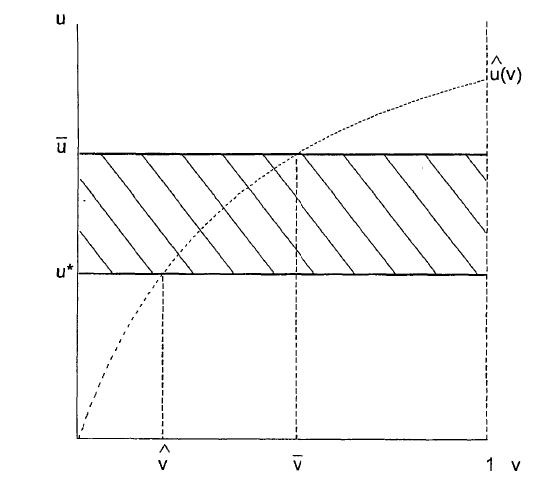
\includegraphics[width=8cm]{Repullo2000DI.png}
\caption{Optimal allocation of LLR powers. Source: \protect\cite{repullo2000}.}
\label{fig:RepDI}
\end{centering}
\end{figure}

\newpage
\appendix
\section{Mathematical notes Repullo}
To obtain the optimal allocation of LLR responsibilities the different welfare cost functions are compared and the optimal one is chose. The first welfare cost function when the central bank is LLR is shown in \autoref{eqa1}
\begin{equation}\label{eqa1}
\hat{L}(v)=\int_{u*}^{\hat{u}(v)}[u(R+c)-L]\mathrm{d}F(u)
\end{equation}
Similarly the welfare cost of choosing the deposit insurance corporation as LLR is given by \autoref{eqa2}
\begin{equation}\label{eqa2}
\hat{L}(v)=\int_{u*}^{\bar{u}}[u(R+c)-L]\mathrm{d}F(u)
\end{equation}

\bibliographystyle{apacite}
\bibliography{bibliography}

\end{document}